
\section{Experiments}
\label{sec:experiments}

We evaluate video quality, continuous control, and multi-query cost. We also
test unseen controls, encoder variants, and reconstruction error. Main results
use held-out objects or actors, three seeds, and 50 denoising steps.

\begin{table*}[t]
\centering
\caption{\textbf{Results on held-out objects and actors.} Values are averaged
over five OpenIllumination folds or four MEAD folds, with three seeds and
50 denoising steps. Trajectories and DiT calls are counted per video family.
The best and second-best fidelity or ordering values are bold and underlined
within each dataset.}
\label{tab:main_results}
\footnotesize
\setlength{\tabcolsep}{4.0pt}
\begin{tabular}{llrrrrrr}
\toprule
Dataset & Method & LPIPS$\downarrow$ & PSNR$\uparrow$ & SSIM$\uparrow$ & $\rho\uparrow$ & Traj. & DiT calls \\
\midrule
\multirow{4}{*}{Lighting}
 & Pointwise independent  & \underline{.3979} & \underline{19.69} & \underline{.737} & .468 & 9 & 450 \\
 & Pointwise shared-noise & .4000 & 19.29 & .731 & .786 & 9 & 450 \\
 & Endpoint interpolation & .4059 & 19.33 & .727 & \underline{.860} & 2 & 100 \\
 & LFVD                   & \textbf{.3216} & \textbf{21.14} & \textbf{.753} & \textbf{.933} & \textbf{1} & \textbf{50} \\
\midrule
\multirow{4}{*}{MEAD}
 & Pointwise independent  & \textbf{.1063} & \textbf{22.97} & \textbf{.764} & .577 & 3 & 150 \\
 & Pointwise shared-noise & .1157 & 22.54 & .753 & \underline{.743} & 3 & 150 \\
 & Endpoint interpolation & .1152 & \underline{22.91} & \underline{.762} & \textbf{.859} & 2 & 100 \\
 & LFVD                   & \underline{.1151} & \textbf{22.97} & .760 & .719 & \textbf{1} & \textbf{50} \\
\bottomrule
\end{tabular}
\end{table*}

\begin{figure*}[t]
\centering
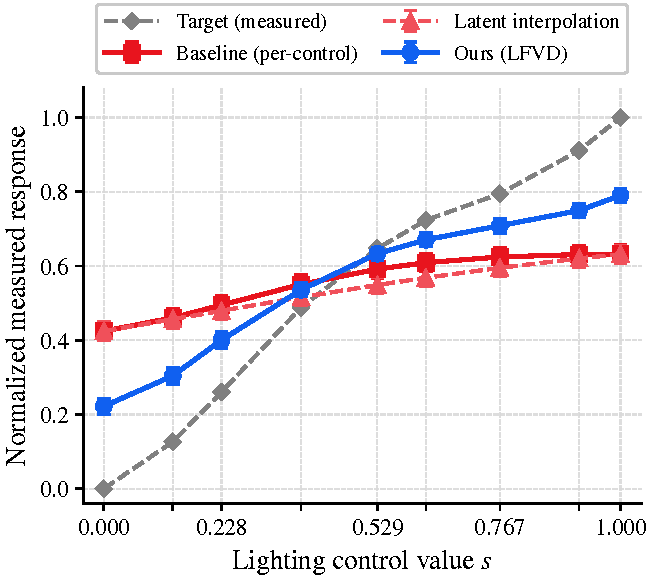
\includegraphics[width=.40\textwidth]{figures/fig3a_lighting_response.pdf}\hspace{.06\textwidth}%
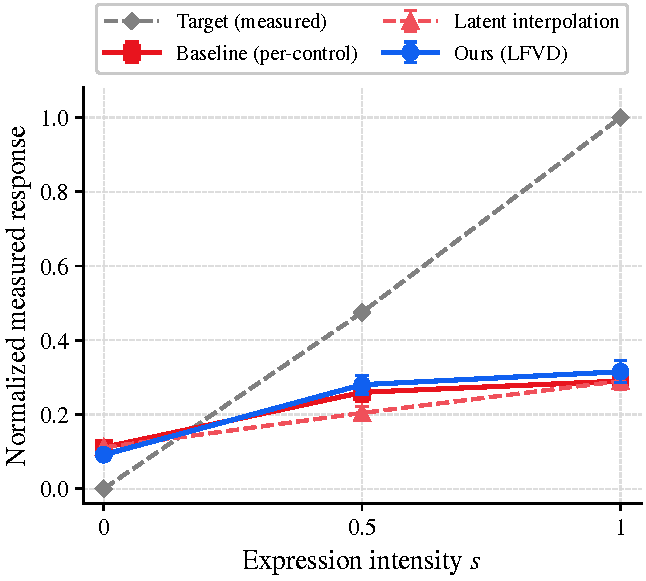
\includegraphics[width=.40\textwidth]{figures/fig3b_mead_response.pdf}
\caption{\textbf{Measured response over the requested control coordinate.}
Curves aggregate the held-out Lighting and MEAD evaluations. LFVD queries
the complete curve after one sampled family code; Pointwise executes a full
trajectory for every coordinate.}
\label{fig:response_curves}
\end{figure*}

\subsection{Experimental Setup}

\paragraph{Datasets.}
\emph{OpenIllumination}~\cite{liu2023openillumination} captures real objects
under one-light-at-a-time illumination. We fix a 17-frame camera path and
vary nine measured light positions, normalized to $s\in[0,1]$ by angular arc
distance. Five object-disjoint folds contain 48/16/16 training, validation,
and test families each, totaling 80 held-out families.

\emph{MEAD}~\cite{wang2020mead} provides facial videos at three ordinal
expression intensities (low, medium, high). We align recordings using dynamic
time warping on mel-frequency cepstral coefficients and their temporal
derivatives, then form 17-frame families. Four actor-disjoint folds use
five training, one validation, and two test actors each, totaling 112
held-out families. MEAD contains identifiable faces and voices. We use this
existing dataset under its research terms and collect no new participant
data; no new IRB review or consent process was conducted.

\paragraph{Implementation.}
We use the Wan2.2-TI2V-5B Video DiT and frozen video
VAE~\cite{wan2025} with the official DiffSynth trainer. All videos have 17 RGB
frames at $256\times256$ resolution. We train the family encoder and query
decoder for 8,000 updates, freeze them, and train rank-64 LoRA adapters on
Video DiT attention and MLP projections for 3,456 updates. Pointwise models
use the same backbone, optimizer, LoRA rank, number of updates, splits, and
conditioning. Sampling uses 50 steps with seeds $\{100,200,300\}$.

\paragraph{Baselines.}
\emph{Pointwise independent} samples each control value with independent
Gaussian noise. \emph{Pointwise shared-noise} uses the same initial noise for
all requested values and runs a complete denoising process for each value.
\emph{Endpoint interpolation} generates the two endpoint videos and linearly
interpolates their VAE latents. Unless specified otherwise, LFVD denotes
LFVD-Mix. We also evaluate LFVD-Identity and LFVD-Compact.

\paragraph{Metrics.}
We report AlexNet LPIPS~\cite{zhang2018lpips}, PSNR, and SSIM against
measured targets. Control correlation $\rho$ is the Spearman correlation
between $s$ and the target-projected response; constant outputs receive zero.
Endpoint amplitude measures response range, and path second variation
measures smoothness. We use paired object- or actor-level cluster bootstrap
intervals (95\%). Full settings and per-sample results are in the supplement.

\subsection{Main Results}

% Four-example method comparison matching MotionStone Fig. 4 geometry.
\begin{figure*}[t]
\centering
\qsetupwide{\dimexpr(\textwidth-13pt)/2-\qL-2pt\relax}%
\qpanel{%
  \qtitle{\textbf{(a) Lighting}\enspace{\color{qgray}held-out object 335, $s{=}.529$}}
  \qframevalues{4}{8}{12}{16}
  \qrowtight{black}{\scriptsize Target}{\qimg{lighting_L3_f013_s100_m0_s04_motionstone.png}}
  \qrowtight{qgray}{\scriptsize Pointwise}{\qimg{lighting_L3_f013_s100_m2_s04_motionstone.png}}
  \qrowtight{qgray}{\scriptsize Endpoint interp.}{\qimg{lighting_L3_f013_s100_m3_s04_motionstone.png}}
  \qrowtight{qblue}{\scriptsize\bfseries LFVD}{\qimghl{lighting_L3_f013_s100_m4_s04_motionstone.png}}
}\hfill{\color{black!25}\vrule width .4pt}\hfill
\qpanel{%
  \qtitle{\textbf{(b) Lighting}\enspace{\color{qgray}held-out object 318, $s{=}.529$}}
  \qframevalues{4}{8}{12}{16}
  \qrowtight{black}{\scriptsize Target}{\qimg{lighting_L3_f010_s100_m0_s04_motionstone.png}}
  \qrowtight{qgray}{\scriptsize Pointwise}{\qimg{lighting_L3_f010_s100_m2_s04_motionstone.png}}
  \qrowtight{qgray}{\scriptsize Endpoint interp.}{\qimg{lighting_L3_f010_s100_m3_s04_motionstone.png}}
  \qrowtight{qblue}{\scriptsize\bfseries LFVD}{\qimghl{lighting_L3_f010_s100_m4_s04_motionstone.png}}
}%
\par\vspace{5pt}
{\color{black!25}\hrule height .4pt}\vspace{5pt}%
\qpanel{%
  \qtitle{\textbf{(c) MEAD}\enspace{\color{qgray}M003 happy-002, $s{=}.5$}}
  \qframevalues{2}{6}{10}{14}
  \qrowtight{black}{\scriptsize Target}{\qimg{mead_M0_f008_s100_m0_s01_motionstone.png}}
  \qrowtight{qgray}{\scriptsize Pointwise}{\qimg{mead_M0_f008_s100_m2_s01_motionstone.png}}
  \qrowtight{qgray}{\scriptsize Endpoint interp.}{\qimg{mead_M0_f008_s100_m3_s01_motionstone.png}}
  \qrowtight{qblue}{\scriptsize\bfseries LFVD}{\qimghl{mead_M0_f008_s100_m4_s01_motionstone.png}}
}\hfill{\color{black!25}\vrule width .4pt}\hfill
\qpanel{%
  \qtitle{\textbf{(d) MEAD}\enspace{\color{qgray}M005 angry-015, $s{=}.5$}}
  \qframevalues{1}{7}{12}{16}
  \qrowtight{black}{\scriptsize Target}{\qimg{mead_M0_f020_s200_m0_s01_motionstone.png}}
  \qrowtight{qgray}{\scriptsize Pointwise}{\qimg{mead_M0_f020_s200_m2_s01_motionstone.png}}
  \qrowtight{qgray}{\scriptsize Endpoint interp.}{\qimg{mead_M0_f020_s200_m3_s01_motionstone.png}}
  \qrowtight{qblue}{\scriptsize\bfseries LFVD}{\qimghl{mead_M0_f020_s200_m4_s01_motionstone.png}}
}%
\par\vspace{-3pt}
\caption{\textbf{Qualitative comparison on held-out Lighting and MEAD families.}
Rows show the measured target, shared-noise Pointwise, endpoint latent
interpolation, and LFVD (blue frame); columns show temporal frames. The top
row contains two Lighting objects and the bottom row two MEAD expressions.
Endpoint interpolation can leave soft double contours in (d), whereas LFVD
produces a coherent facial trajectory. All panels use the locked 50-step test
protocol without sharpening, alignment, or color correction.}
\label{fig:main_qualitative}
\end{figure*}


On OpenIllumination (Table~\ref{tab:main_results}), LFVD improves LPIPS
from .4000 to .3216, PSNR from 19.29 to 21.14 dB, and correlation from
.786 to .933 relative to shared-noise Pointwise. It uses one trajectory
for nine values, compared with nine for Pointwise. LFVD's 95\% object-level
intervals are $[.3096,.3344]$ (LPIPS), $[20.58,21.65]$ dB (PSNR), and
$[.905,.960]$ (correlation). Shared noise yields higher Pointwise correlation
than independent noise (.786 versus .468).

On MEAD, LFVD matches shared-noise Pointwise fidelity (.1151 versus .1157
LPIPS) but has lower correlation (.719 versus .743). Endpoint interpolation
reaches .859 correlation, despite LFVD's larger endpoint response. These
results show different fidelity and ordering behavior across control domains.
Figure~\ref{fig:response_curves} plots the measured response over $s$.
Figure~\ref{fig:main_qualitative} compares methods on two held-out Lighting
objects and two held-out MEAD families across selected temporal frames.
Endpoint latent interpolation can produce soft double facial contours, or
ghosting, from blending endpoint states; this is most visible for M005
angry-015 in Figure~\ref{fig:main_qualitative}(d). The selected examples expose
method differences, while Table~\ref{tab:main_results} remains the aggregate
test.
Figure~\ref{fig:control_sweeps} shows Lighting continua decoded from a single
LFVD trajectory.

% Control sweeps decoded from one LFVD trajectory (MotionStone Fig. 5/6 style).
\begin{figure*}[t]
\centering
\qsetup{\dimexpr(\textwidth-13pt)/2-\qL-2pt\relax}%
\qpanel{%
  \qtitle{\textbf{(a) Lighting}\enspace{\color{qgray}held-out object 318}}
  \qframes
  \qrow{qorange}{\scriptsize\boldmath$s{=}0.000$}{\qimg{lighting_L3_f010_s100_m4_s00.png}}
  \qrow{qorange}{\scriptsize\boldmath$s{=}0.529$}{\qimg{lighting_L3_f010_s100_m4_s04.png}}
  \qrow{qorange}{\scriptsize\boldmath$s{=}1.000$}{\qimg{lighting_L3_f010_s100_m4_s08.png}}
}\hfill{\color{black!25}\vrule width .4pt}\hfill
\qpanel{%
  \qtitle{\textbf{(b) Lighting}\enspace{\color{qgray}held-out object 308}}
  \qframes
  \qrow{qorange}{\scriptsize\boldmath$s{=}0.000$}{\qimg{lighting_L3_f008_s100_m4_s00.png}}
  \qrow{qorange}{\scriptsize\boldmath$s{=}0.529$}{\qimg{lighting_L3_f008_s100_m4_s04.png}}
  \qrow{qorange}{\scriptsize\boldmath$s{=}1.000$}{\qimg{lighting_L3_f008_s100_m4_s08.png}}
}%
\par\vspace{-3pt}
\caption{\textbf{Continuous control from one LFVD trajectory.} In each panel,
all rows are decoded from one sampled family code at different control values
$s$ (orange); columns are temporal frames. Both panels show held-out
OpenIllumination objects at three measured light coordinates. No query
requires an additional Video DiT call.}
\label{fig:control_sweeps}
\end{figure*}


\subsection{Generalization to Unseen Controls}
\label{sec:sparse_control}

We train Pointwise and LFVD-Mix using only three OpenIllumination positions,
with indices $\{0,4,8\}$, and evaluate all nine measured positions. The six
intermediate positions are excluded from both codec and diffusion training.
We use the same five object-disjoint test folds, three seeds, and 50-step
sampling. All targets are recorded measurements.

\begin{table}[t]
\centering
\caption{\textbf{Lighting control with three training positions.} Observed
values are used in training; unseen values are the six remaining measured
positions. Results cover five folds, three seeds, and 50 steps.}
\label{tab:sparse_control}
\footnotesize
\setlength{\tabcolsep}{3.2pt}
\begin{tabular}{llrrr}
\toprule
Subset & Method & LPIPS$\downarrow$ & PSNR$\uparrow$ & SSIM$\uparrow$ \\
\midrule
Observed & Pointwise shared & .4062 & 18.48 & .7181 \\
         & LFVD-Mix         & \textbf{.2993} & \textbf{20.99} & \textbf{.7532} \\
Unseen   & Pointwise shared & .4103 & 18.81 & .7232 \\
         & LFVD-Mix         & \textbf{.3410} & \textbf{21.22} & \textbf{.7480} \\
\bottomrule
\end{tabular}
\end{table}

On unseen positions (Table~\ref{tab:sparse_control}), LPIPS improves from
.4103 to .3410 and PSNR from 18.81 to 21.22 dB. Across 80 test families,
20 objects, and three seeds, paired gains are .0693 LPIPS (95\% CI
$[.0576,.0825]$), 2.41 dB PSNR ($[2.13,2.69]$), and .0248 SSIM
($[.0191,.0305]$). Correlation over all nine values rises from .604 to
.991, a gain of .386 ($[.316,.464]$).

\subsection{Family Encoder Ablation}
\label{sec:encoder_ablation}

Identity and Mix are statistically tied on full-grid Lighting (LPIPS
difference, Identity minus Mix: $-.0014$, 95\% CI $[-.0058,.0030]$) and
sparse unseen controls ($+.0007$, $[-.0015,.0028]$). On MEAD, Identity has
lower LPIPS by .0082 ($[.0002,.0204]$) and higher PSNR by .19 dB
($[.00,.46]$). Thus the family-valued formulation is robust to the encoder
choice, while learned mixing is not uniformly beneficial. The supplement
reports complete encoder metrics and paired intervals for both datasets.

\subsection{Measured Multi-Query Cost}
\label{sec:cost}

As defined in Eq.~\ref{eq:generation_cost}, Pointwise repeats
$\mathcal C_{\mathrm{diff}}(T_z)$ for each requested video, while LFVD pays
$\mathcal C_{\mathrm{diff}}(1+J')$ once and adds a query cost for each
output. We compare both sequential Pointwise and batch-3 Pointwise, the
strongest memory-feasible baseline. The supplementary timing curve and table
report synchronized wall-clock time on one RTX 4090.

In Lighting, the measured crossover occurs at approximately seven queries:
LFVD takes 15.40 s at $M=7$, compared with 16.96 s for batch-3 Pointwise.
At $M=9,17,33$, LFVD is 1.23$\times$, 1.97$\times$, and 2.90$\times$
faster than batched Pointwise. For MEAD's three control values, LFVD takes
5.74 s, compared with 6.60 s for batch-3 Pointwise and 11.47 s for
sequential Pointwise.

The supplementary FLOP audit reports patch and text projections, attention
projections and products, and feed-forward layers.
Each multiply--accumulate is counted as two FLOPs. The diffusion-only
crossover is 2.37 queries for MEAD and 6.82 for Lighting. At $M=7$,
Lighting Pointwise requires 1,214.47 TFLOPs, compared with 1,183.59
TFLOPs for LFVD; at $M=9$, the ratio is 1.32$\times$. These analytical
results exclude query and VAE decoding and complement the measured timings.
The sparse Lighting model uses 13 latent frames, 64.9\% fewer than the
37-frame dense model. Its LPIPS over all nine queried values is .3271,
compared with .3216 for the dense model, and its transformer-only crossover
is 2.37 queries.

\subsection{Ablations and Bottleneck Analysis}

Exact-code decoding reaches .0642 LPIPS and perfect ordering, close to the
frozen VAE floor of .0512; sampling the same representation raises LPIPS to
.3365. Family-code diffusion, rather than the query decoder, is therefore
the main quality bottleneck. Rank, training-family scaling, and coordinate
ablations support the same conclusion. LFVD-Compact shortens the code from
37 to 28 frames and moves the analytical crossover from 6.82 to 5.09
queries, but degrades sampled LPIPS from .3300 to .4053. Complete protocols,
tables, and qualitative decompositions are provided in the supplement.

\subsection{Limitations}

LFVD generates a larger latent representation than a single video and
requires enough queries to amortize its initial cost. OpenIllumination
provides controlled multi-view sequences; MEAD provides native videos but
only three ordinal expression levels, where endpoint interpolation gives
higher ordering correlation. The comparison between Identity and Mix is
small and dataset-dependent, and the Compact variant loses fidelity.
Finally, sampled-code quality remains below exact-code reconstruction,
leaving family-code diffusion as the main limitation of the current model.
